\documentclass[12pt,a4paper]{article}

\usepackage[left=1in,right=1in,top=1in,bottom=1in]{geometry}                % See geometry.pdf to learn the layout options. There are lots.
\usepackage[parfill]{parskip}    % Activate to begin paragraphs with an empty line rather than an indent
\usepackage{microtype} \hyphenpenalty=750
\usepackage{graphicx}
\usepackage{epstopdf} \DeclareGraphicsRule{.tif}{png}{.png}{`convert #1 `dirname #1`/`basename #1 .tif`.png}
% \usepackage[applemac]{inputenc}
\usepackage{booktabs}
% \usepackage{fancyhdr} \pagestyle{fancy} \chead{\hifibau} \cfoot{\thepage}
% \usepackage[english,ngerman]{babel}

\usepackage{siunitx}

\PassOptionsToPackage{hyphens}{url}\usepackage[colorlinks]{hyperref}
\usepackage{caption} \captionsetup{labelfont={sf,bf}, size=footnotesize}

\usepackage[superscript,biblabel]{cite}

% set format of document title
\usepackage{titling}
\pretitle{\begin{center}\Large\bfseries}
\posttitle{\end{center}\vspace{1em}}
\preauthor{\begin{center}\large}
\postauthor{\end{center}\vspace{1em}}
\predate{\begin{center}\large}
\postdate{\end{center}\vspace{1em}}

% set formats of section headings
\usepackage[explicit]{titlesec}
\titleformat{\title}{\centering}{\thesection.}{0.5em}{\MakeUppercase{#1}}
%\titleformat{\section}{\centering}{\thesection.}{0.5em}{\MakeUppercase{#1}}
\titleformat{\section}{}{\thesection.}{0.5em}{\MakeUppercase{#1}}
%\titleformat{\subsection}[runin]{\slshape}{\thesubsection.}{0.5em}{#1. }
\titleformat{\subsection}{\slshape}{\thesubsection.}{0.5em}{#1 }
\titleformat{\subsubsection}[runin]{\slshape}{\thesubsubsection.}{0.5em}{#1. }
 
\usepackage[T1]{fontenc} \usepackage[scaled=.90]{helvet} \renewcommand{\familydefault}{\sfdefault} \usepackage[helvet]{sfmath}

\newcommand{\Ohm}{\ensuremath{\Omega}}
\sisetup{detect-all} % tell siunitx to detect font stuff


% \setlength{\columnsep}{0.75cm} 

\graphicspath{{figures/}}

% \interfootnotelinepenalty=10000

\providecommand{\figr}[1]{Fig.~\ref{fig:#1}}
\providecommand{\figlabel}[1]{\label{fig:#1}}
\providecommand{\tabl}[1]{Tab.~\ref{tab:#1}}
\providecommand{\tablabel}[1]{\label{tab:#1}}
\providecommand{\secn}[1]{Sec.~\ref{sec:#1}}
\providecommand{\seclabel}[1]{\label{sec:#1}}


%% define formats of section and subsection etc. headings:
%    \makeatletter
%    \def\section{\@startsection{section}{1}%
%    \z@{.7\linespacing\@plus\linespacing}{.5\linespacing}%
%%    {\normalfont\bfseries\centering}}
%    {\Large\centering}}
%    
%    \def\subsection{\@startsection{subsection}{2}%
%    \z@{.5\linespacing\@plus.7\linespacing}{-.5em}%
%%    {\normalfont\bfseries\itshape}}
%    {\normalfont\itshape}}
%    
%    \def\subsubsection{\@startsection{subsubsection}{3}%
%    \z@{.5\linespacing\@plus.7\linespacing}{-.5em}%
%%    {\normalfont\bfseries}}
%    {\normalfont\itshape}}
%    
%    \makeatother






\title{The Open-Source Directly-Heated Triode \\ Electrostatic Headphone Amplifier \\ (OSDEHA)}
\author{Matthias Brennwald}
\date{THIS DOCUMENT IS UNDER CONSTRUCTION!\\ Draft Version \today}

\begin{document}

% \twocolumn[\maketitle]

\maketitle

\emph{Warning: This DIY project involves high voltage. Individuals utilizing the information provided must possess expert knowledge, adhere to stringent safety precautions, and accept all risks associated with electrical work. The authors and contributors of this project expressly disclaim any liability for injuries or damages arising from the use or misuse of this information.}


\section{Overview}

This document describes an audio amplifier for electrostatic headphones. The design of the amplifier is targeted at DIY builders and is published as open hardware (see \secn{license}).

Electrostatic headphones operate on audio signals characterized by high voltage and low current. This is the domain of vacuum tubes, making them most suitable as drivers for e-stats.  While there exist a number of tube amplifiers for e-stat headphones, many of these designs do not utilize directly-heated triodes (DHTs), which exhibit outstanding linearity and sound quality.\par

The OSDEHA uses DHT tubes for its output stage and implements the following design goals:
\begin{itemize}
\item The audio output is taken directly from the anodes of the DHT output tubes. There are no transformer or capacitors to transfer the power to the headphones.
\item The amplifier input takes balanced input at signal levels of modern audio sources (mostly DACs these days).
\item The design prioritizes the quality of audio reproduction and electronic design rather than on low cost.
\item The amplifier should be reasonably compact, and all units and boards should fit in one single chassis.
\end{itemize}

There is a public discussion thread of the OSDEHA at diyAudio\cite{osdeha_p1}. 

\section{Amplifier Circuit}

\subsection{Driving electrostatic headphones} \seclabel{estat_drive}

Electrostatic headphones utilize three electrodes: two fixed outer electrodes (stators) and a movable central electrode (diaphragm). The diaphragm is biased at a high voltage relative to the stators. The audio signal is applied to the stators in opposite polarities, creating an electric field that controls the movement of the charged diaphragm. For accurate sound reproduction, the electrostatic forces acting on the diaphragm must be proportional to the applied audio signal. To avoid distortion of the audio output from the headphone, the charge on the diaphragm therefore needs to be maintained constant.

The electrical impedance of electrostatic headphones is primarily determined by the capacitance of the two stators, which is typically around \SI{100}{pF}\cite{osdeha_p3}.

The voltage swing to drive the stators depends on the headphone sensitivity and the desired sound pressure level. An experiment using various genres of well-recorded music indicated that an undistorted \SI{1.3}{kV} peak-to-peak swing of the bipolar output is desirable (i.e., \SI{650}{V} peak-to-peak at each stator)\cite{osdeha_p8}. The corresponding current swing measured in this experiment was approximately \SI{4}{mA}, but driving the \SI{100}{pF} load to full output at \SI{20}{kHz} and higher necessitates larger peak currents, around \SI{20}{mA}\cite{osdeha_p2}.

% With a balanced line-level input ($2\times\SI{3.5}{V}$ peak-to-peak), the required voltage gain of the amplifier is $1300/(2\times 3.5) = 185\times$, or \SI{+45}{dB}.

\subsection{Output Stage}\seclabel{outputstage}

\figr{OPS_concept} shows the conceptual layout of the OSDEHA. The output stage uses two DHTs in a push-pull arrangement to provide the symmetric, bipolar output needed to drive electrostatic headphones. For efficient transfer of the audio power to the headphones, the AC impedance of the anode loads must be larger than that of the headphones (several \unit{M\Ohm}). This cannot be implemented with passive anode-load resistors, so active constant-current sources (CCSs) are used in this position. The CCS loads also improve the linearity and voltage gain of the amplifier, and suppress ripple and noise from the B+ rails.

\begin{figure}
\begin{center}
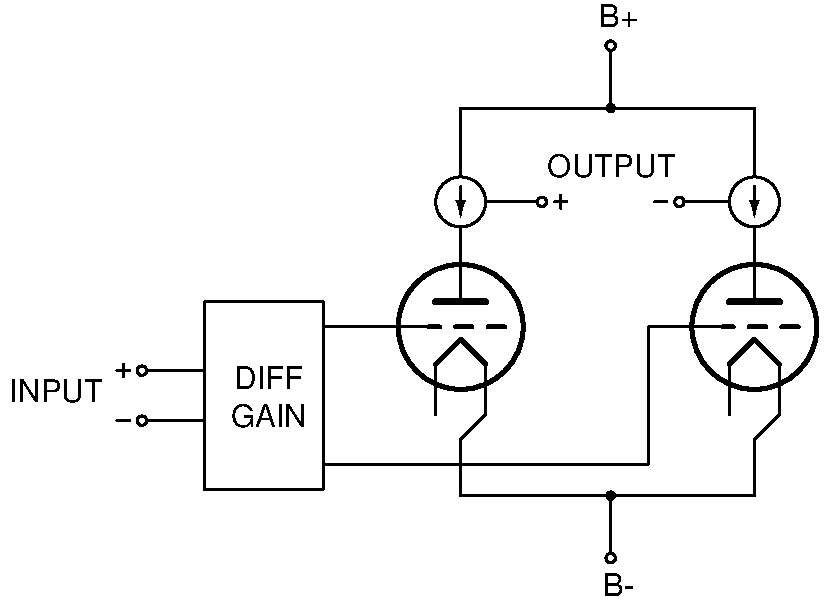
\includegraphics[width=0.7\textwidth]{OPS_concept.pdf}
\caption{Conceptual layout of the OSDEHA: differential input, gain stage stage, and push-pull DHT output stage.}
\figlabel{OPS_concept}
\end{center}
\end{figure}

The DC level of the amplifier differential output should be close to \SI{0}{VDC}. The absolute DC voltage of the output nodes should be approximately at GND, centered between B+ and B-. The CCS loads, therefore, need to drop the DC voltage from B+ to approximately \SI{0}{VDC}, and the DHT tubes drop the remaining voltage to B-. The output DC voltages could be zeroed by adjusting the biasing of the tubes accordingly, but this would be prone to drift of the output tubes. Better control of the output DC is achieved by using a ``gyrator'' circuit as conceived by Ale Moglia\cite{mogliaa_gyrator} (\figr{gyrator_concept}). The ``gyrator'' works as a CCS in the audio/AC domain, but provides a fixed DC voltage to bias the tube anode close to GND and thus maintains the output DC voltage despite any thermal drift or aging of the DHT tubes.

\begin{figure}
\begin{center}
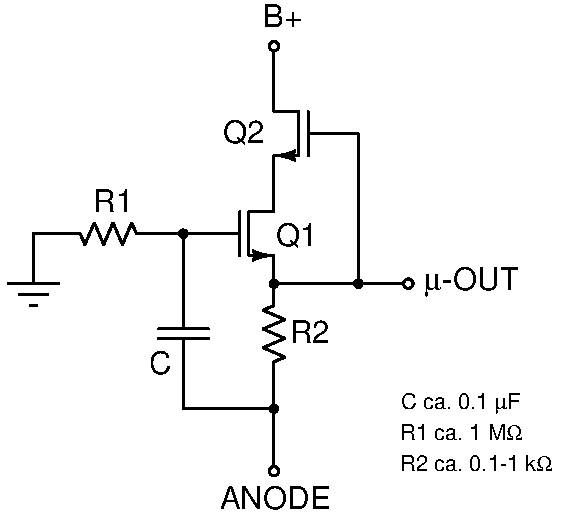
\includegraphics[width=0.45\textwidth]{gyrator_concept.pdf}
\caption{``Gyrator'' circuit (simplified). At DC, the gate pin of the FET Q1 is grounded at \SI{0}{V} via R1, and the source pin is fixed at $-V_{\rm GS,0}$. The anode voltage is determined by the DC drop across R2, which in turn depends on the anode DC bias current as determined by the bias voltage applied to the grid of the tube. The depletion-mode FET Q2 drops most of the voltage from B+ to the anode and decouples Q1 from any noise or ripple on B+. At AC, the gate voltage of Q1 is tied to the anode through capacitor C, and Q1 and R2 operate as a CCS. If the audio output to the stator is taken from the $\mu$-output, the anode receives the full CCS output and the DHT therefore operates at a constant current that is independent of the stator current.}
\figlabel{gyrator_concept}
\end{center}
\end{figure}

The choice of the output tube type is determined by the drive requirements for the headphone, as described in \secn{estat_drive}. Since the two tubes are in series with the headphone, each tube contributes half of the total voltage swing. Each tube needs to swing \SI{\pm325}{V} at a \SI{20}{mA} bias. Additionally, to emphasize the ``DHT sound,'' the DHT output stage should contribute as much voltage gain as possible to the overall gain of the amplifier.

Several DHT tube types were considered for the OSDEHA\cite{osdeha_p9,osdeha_whichDHT}. In particular:

\begin{itemize}
\item The 841/VT-51 tube has a gain of 30$\times$ and can be biased up to \SI{425}{V}. However, at the operating point required for the OSDEHA, the 841 tends to operate at a positive grid voltage, which leads to grid current draw. Moreover, these tubes are relatively scarce.
\item The 20B tube is a modern design with a gain of 20$\times$, the 20B can be biased up to about \SI{500}{V}. However, these tubes are quite large (approximately the size of a beer bottle) and are manufactured in small quantities by a single producer (Emissionlabs), making their long-term availability uncertain.
\item The family of the 801/801A/VT-62 and 10Y/VT-25 types\cite{aasyl_801types} provide a gain of 8$\times$. The 801 can be biased up to \SI{500}{V}, while the 10Y should not be biased above \SI{450}{V}. These tubes are available as new-old-stock and from new production.
\end{itemize}

From a technical standpoint, the high gain of the 20B would would make this tube an interesting option. However, due to concerns about the long-term availability of the 20B, the 801/10Y family of tubes is considered a more practical choice for the OSDEHA design.

\figr{801A_curves} shows the characteristic curves measured from the 801A tube (the 10Y/VT-25 are equivalent) with the load line of a \SI{20}{mA} CCS. The anode DC bias is set at \SI{440}{V}, corresponding to a grid bias of approximately \SI{-37}{V}. This bias point facilitates an anode voltage swing of \SI{\pm325}{V} within the linear operating range of the tube. Additionally, the grid voltage does not exceed +\SI{5}{V}, where the grid current has been measured to stay well below \SI{1}{mA}.


\begin{figure}
\begin{center}
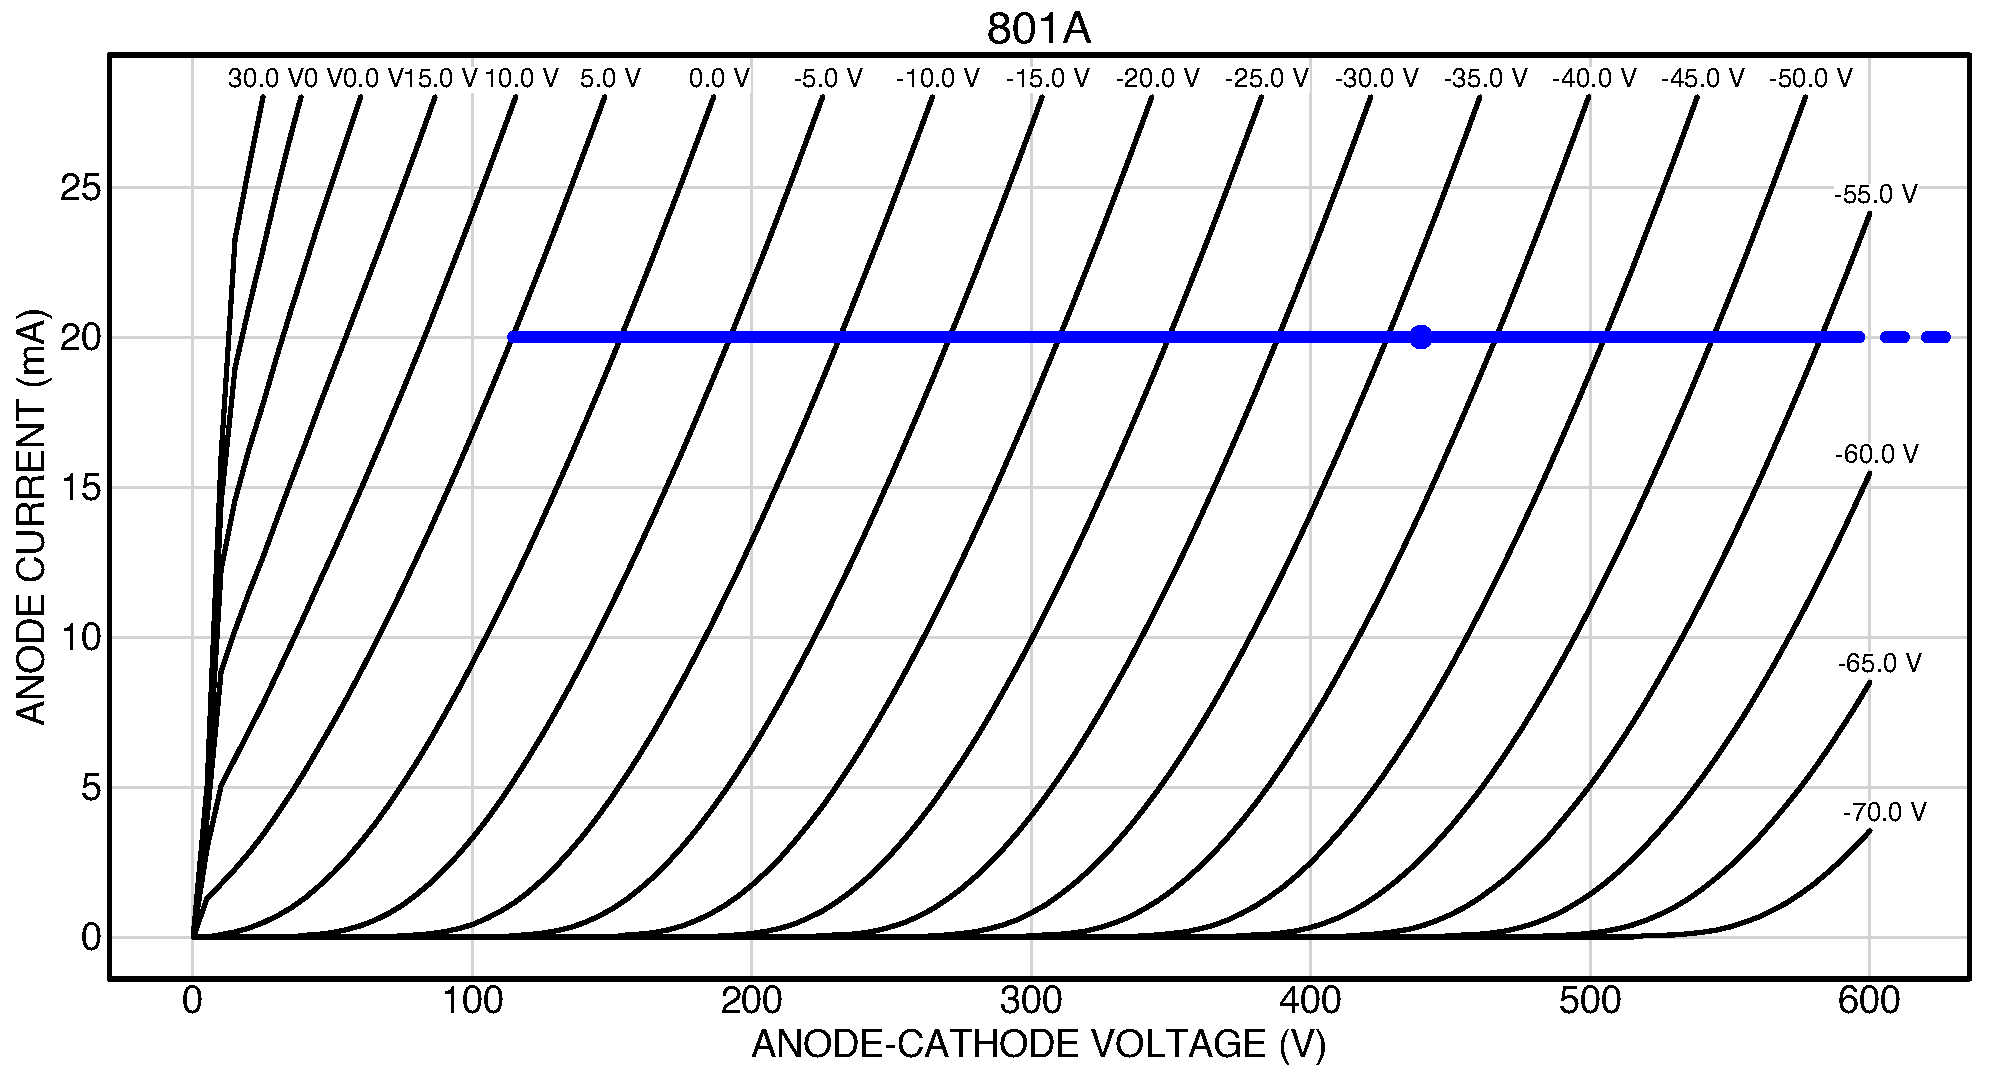
\includegraphics[width=\textwidth]{801A_curves.pdf}
\caption{Characteristic curves measured from an 801A DHT, with \SI{20}{mA} CCS load line and a \SI{440}{V} bias and a \SI{\pm325}{V} anode swing (blue).}
\figlabel{801A_curves}
\end{center}
\end{figure}


The constant current AC output from each CCS is shared between the DHT and the headphone stator. The current flowing through the DHT will therefore exhibit a slight variation in response to the AC current draw by the stator. However, this AC current variation will be small (less than \SI{4}{mA})\cite{osdeha_p8}, and the general concept for the operating point illustrated in \figr{801A_curves} remains valid. The ``gyrator'' can also be configured to operate as a $\mu$-follower\cite{pimm_ccs,kimmel_mustage}, if the stator current is taken directly from the source pin of the ``gyrator'' FET. This configuration restores the constant-current operation of the DHT tube with a perfectly flat load line exactly as shown in \figr{801A_curves}.



\subsection{Input Stage}\seclabel{inputstage}

Following the lines of the output stage, the differential input stage is designed as a symmetric long-tailed pair (LTP)\cite{valvewizard_LTP} using tubes with triode characteristics. The linearity and the voltage gain of the LTP is optimized with a very high AC impedance of the ``tail'', which is implemented as a CCS.

The input stage needs to provide the voltage gain to drive the grids of the output tubes with an AC amplitude of $2 x \SI{86}{V}$ (peak-to-peak, \figr{801A_curves}). With a balanced line-level peak-to-peak input of $2 x \SI{3.5}{V}$, a voltage gain of $86 / 3.5 = 25\times$ is needed. The E180F or 6E5P tubes connected as triodes provide suitable gain and offer very linear amplification \cite{bartola_thdbenchmark,millett_pentodes,klausmobile_testerfiles}. However, the E180F tends to be microphonic\cite{osdeha_p23} and the 6E5P exhibits better linearity than the E180F\cite{osdeha_p32}, making the 6E5P the preferred choice for the LTP input stage.



------------
COUPLING AND BUFFERING TO OUTPUT STAGE DHT GRIDS: The grids of the output tubes will be biased below the B- / -HV rails, so it would be rather complicated to DC couple the LTP input/driver stage to the output stage. Capacitor coupling works very well [https://linearaudio.net/cyril-batemans-capacitor-sound-articles], especially if there is no substantial current flowing through the capacitor. Driving the output stage into A2 therefore needs a current buffer. A MOSFET source follower should do the trick.
------------


\section{Power supplies}

\subsection{High voltage supplies (B+, B-, B2-)}

\subsection{Bias}

\subsection{DHT filament supply}

\subsection{Heater supply for input stage}


\section{License information} \seclabel{license}
Copyright Matthias Brennwald 2024.                                                    

The OSDEHA is Open Hardware and is licensed under the CERN-OHL-S v2 or any later version.

You may redistribute and modify this source and make products using it under the terms of the CERN-OHL-S v2 (\url{https://ohwr.org/cern_ohl_s_v2.txt}).

This source is distributed WITHOUT ANY EXPRESS OR IMPLIED WARRANTY, INCLUDING OF MERCHANTABILITY, SATISFACTORY QUALITY AND FITNESS FOR A PARTICULAR PURPOSE. Please see the CERN-OHL-S v2 for applicable conditions.

Source location: \url{https://github.com/mbrennwa/OSDEHA}

As per CERN-OHL-S v2 section 4, should You produce hardware based on this source, You must where practicable maintain the Source Location visible on the external case of the OSDEHA or other products you make using this source.            

% list of references
\bibliographystyle{unsrt}
\bibliography{OSDEHA_documentation}


\end{document}
